\chapter{Datamanagement}
\label{chap:datamanagement}
Deze lessen gaan over het importeren, opslaan, verwerken, en aanpassen van data voor later gebruik.

\section{Beheer van gegevens}
Of je nou analyses uitvoert, polymeren onderzoekt, nanotechnologisch bezig bent: als chemicus ben je constant bezig om data te verkrijgen, te verwerken, en te interpreteren. 

Een van de belangrijkste dingen hierbij is dat data systematisch wordt opgeslagen in een vorm die ook later nog bruikbaar is. De eerste les van dit onderdeel gaat hierover: welke technieken zijn er om je gegevens te beheren?

In dit onderdeel houden we het bij relatief simpele voorbeelden: gegevens die overzichtelijk in excel-sheets passen en die door 1 persoon worden beheerd en gebruikt. Voor meer ingewikkelde gevallen heb je vaak databases nodig, om bijvoorbeeld grote hoeveelheden data te beheren of om meerdere personen op verschillende manieren toegang te kunnen verlenen. Databases komen aan bod in hoofdstuk~\ref{chap:gegevensbeheer}: Gegevensbeheer.

Voor het opslaan van data maak je van tevoren een plan, die je eventueel aanpast indien nodig. Het maken van een datamanagentsplan (DMP) is verplicht in veel sectoren: onderzoekers moeten bijvoorbeeld zo'n plan aanleveren bij de aanvraag van onderzoeksgeld. Er zijn een heleboel manieren om een dergelijk plan te maken. In dit hoofdstuk wordt er 1 manier doorgewerkt. Het is de bedoeling dat jullie ook een DMP maken voor jullie project Chemical Fingerprinting (en later ook voor Urban Mining).

Een datamanagementsplan bestaat uit verschillende aspecten. Hieronder worden de mogelijke onderdelen besproken, en er wordt meer informatie gegeven over technische aspecten. Vervolgens zal je een voorbeeldcase uitgewerken. In Appendix~\ref{ap:dmp} staat een sjabloon voor het maken van een DMP. 
\begin{itemize}
    \item \textbf{Algemene info}: Het plan bevat een voorblad met de meest essentiële informatie. Denk hierbij aan deelnemers (personen en organisaties), tijdsduur, datum, titel project, taken en rollen van personen
    \item \textbf{Verzamelen}: welk type data wordt er gegenereerd, hoe wordt deze verkregen, in welk formaat, de geschatte grootte van de dataset, de geschatte kosten, en of alles binnen wetgeving valt
    \item \textbf{Documentatie}: in welk format wordt de data opgeslagen, moeten er nog extra documenten bij met uitleg en metadata, in wat voor structuur wordt het opgeslagen, hoe wordt versiebeheer geregeld 
    \item \textbf{Opslag}: wat moet er allemaal worden opgeslagen, waar wordt het opgeslagen, wat zijn de kosten
    \item \textbf{Veiligheid}: is er betrouwbare data bij, wie mag bij welke data, moet data worden opgesplitst in losse sets, wie is de eigenaar van de data, en wat gebeurt er mee na het onderzoek
    \item \textbf{Selectie en behoud}: moet de data voor langere termijn worden bewaard, wie is daar verantwoordelijk voor, hoe wordt dat geregeld, hoe lang moet het worden bewaard
    \item \textbf{Reproductie}: wie mag de data verder gebruiken, welke licentie zit er op de data
\end{itemize}

De meeste onderdelen spreken voor zich. De technische aspecten zijn voor veel van jullie nog nieuw, dus daar wordt wat extra aandacht aan besteed.

\subsection*{Opslag van data}
Als je je bestanden wil opslaan zijn er een boel dingen waar je rekening mee moet houden. Ten eerste moet je weten in welk format je de data verkrijgt. Sommige meetapparaten geven de data in zogenaamde gepatenteerde bestandsformaten. Dit zijn bestanden die je niet zomaar kan openen in andere software. Als je dus je data opslaat op die manier is het mogelijk dat je later deze data niet meer kan openen. Het is dus zaak om te zorgen dat je data wordt opgeslagen op een manier zodat je er altijd bij kan. Bestandsformaten als .csv, .txt, .xlsx, .docx, .zip, zijn open bestandstypes die door erg veel verschillende software geopend kunnen worden. Bestandsformaten als .rar, .psd, .rtf, .wma, zijn gesloten bestandstypes die je alleen met specifieke software kan openen. Vaak is het noodzakelijk om de data van een meetapparaat te exporteren naar een open bestandstype. 

Naast het bestandsformaat is het ook erg handig om een begeleidend document bij de data te plaatsen die uitlegt wat de data precies is, wat de getallen voorstellen, etcetera. Dit wordt ook wel \textit{metadata} genoemd: data die wat zegt over andere data. Denk hierbij bijvoorbeeld aan een .txt bestandje die uitlegt in welke eenheid iedere kolom in een .xlsx bestand is opgeslagen.

Als de data is verzameld en is voorzien van metadata moet het worden opgeslagen. Een gebruikelijke manier is om dit te doen op een USB-stick. Dit is natuurlijk erg fout- en fraudegevoelig: de stick kan kwijtraken of kapotgaan, iedereen met de stick heeft toegang tot de data, er kan maar 1 persoon tegelijkertijd mee werken, etcetera. Dit is dus bijna nooit de goede manier om je data op te slaan.

Tegenwoordig is het bijna altijd standaard om de data op een server van het bedrijf/instelling op te slaan, of in een cloud-opslag zoals Dropbox, Google Drive, of OneDrive. Het is vaak zelfs verplicht om dit te doen om te zorgen dat de data ook voor andere onderzoekers beschikbaar en controleerbaar is, en zodat er automatisch back-ups worden gemaakt van het materiaal.

Hier moet je wel altijd goed nadenken over privacy en toegang. Als je bijvoorbeeld gevoelige informatie wil opslaan wil je niet dat iedere medewerker van je bedrijf daar bij kan, en als je samen wil werken met meerdere instellingen is het soms onmogelijk om dan alles op te slaan op een server van het bedrijf, aangezien niet iedereen daar toegang tot heeft.

In de regel sla je de data altijd op bij de cloud-opslag van je bedrijf, instelling, of school. In ons geval geldt dus dat je alles op gaat slaan op de OneDrive van het Saxion. Hiervoor moet je wel een goede mappen-structuur bedenken om de boel op te slaan: welke indeling wordt er gemaakt, welke bestanden komen erin, welke naamgeving hebben de bestanden, hoe wordt de metadata meegegeven, wie heeft toegang, etcetera. Dit hoort allemaal in je DMP terug te komen. 

\subsection*{Opdracht: Uitwerken datamanagementsplan}
\begin{figure}[h]
\begin{center}
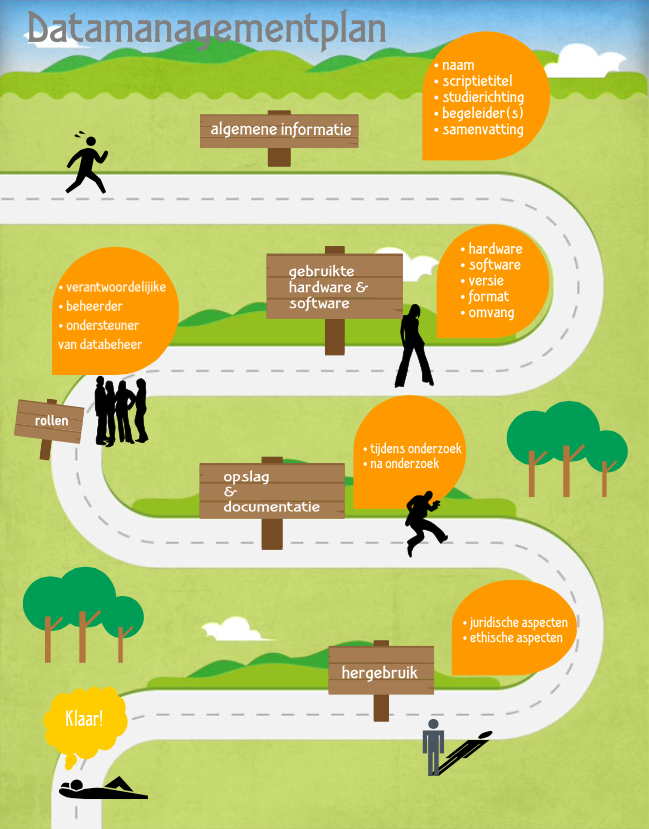
\includegraphics[width=0.6\textwidth]{img/dpm_studenten_infographic.png}
\caption{\label{fig:dmpinfo} \small Infographic voor het opstellen van een DMP. Gebaseerd op een werk van de Universiteitsbibliotheek Nijmegen op \href{http://ru.nl.libguides.com}{\textsf{http://ru.nl.libguides.com}}}
\end{center}
\end{figure}

In dit voorbeeld moet je een DMP opstellen voor een simpel onderzoek. In dit onderzoek worden fipronil-gehaltes bepaald in verschillende monsters. Fipronil is een schadelijke stof die een aantal jaren geleden in eieren terecht is gekomen, wat voor een landelijke herroeping van veel eieren heeft gezorgd. In dit onderzoek worden eieren van verschillende supermarkten onderzocht op fipronil-gehaltes. Het onderzoek wordt uitgevoerd bij het RIKILT (onderdeel van de Nederlandse voedsel- en warenautoriteit) door 2 studenten die daar stage lopen. 

Stap 1 in het DMP is het beschrijven van de algemene informatie:
\begin{table}[h]
\begin{tabular}{ll}
Onderzoekers    & H. van der Steeg, J. van der Maat                    \\
Titel onderzoek & Controleren van de gehaltes fipronil in supermarkteieren \\
Begeleiders     & Dr. B. Swennenhuis                                   \\
Bedrijf        & RIKILT Wageningen                                       \\
Datum      & 1/1/2020 tot 1/4/2020                                            
\end{tabular}
\end{table}

Nu moet er bedacht worden hoe de data wordt verkregen, opgeslagen, wie er verantwoordelijk is, etcetera.

\textbf{Details over het onderzoek}\\
Fipronil is een organisch molecuul wat wordt gemeten met behulp van een GC-MS. De ruwe data komt in .csv bestanden terecht en kan worden geanalyseerd met MSAnalyzer. De verwerkte data wordt opgeslagen als .xls bestand. De bestanden hebben een formaat van maximaal 1 MB per stuk (maar vaak een stuk kleiner). Er worden zo'n 100 eieren gemeten, en van ieder ei wordt zowel het eiwit als het eigeel doorgemeten in duplo. Alle ruwe data moet worden opgeslagen in verband met bewijslast. 

De MS wordt gebruikt om de fipronil-piek te identificeren en de hoogte van de piek in het chromatogram wordt gebruikt om het gehalte te bepalen. De uiteindelijk verwerkte uitkomsten van iedere meting (dus gehalte fipronil) zal in losse bestanden worden opgeslagen. 

De data wordt opgeslagen op de interne servers van het RIKILT. Hier kunnen alleen bevoegde medewerkers van het instituut bij. De bestanden moeten opgeslagen worden inclusief begeleidende tekst in het NL en EN die uitlegt wat er in de bestanden te vinden is en van welke sample de data afkomstig is. 

Er wordt verwacht dat de fipronilconcentratie onder de \SI[per-mode=symbol]{5}{\micro\gram\per\kilo\gram} ligt (maximaal toegestane waarde). Als de waardes hierboven liggen zal er direct melding van worden gemaakt bij de voedsel- en warenautoriteit in verband met een mogelijk gevaar voor de volksgezondheid. Bedrijven kunnen tot 5 jaar na overschrijding van maximale fipronilgehaltes een boete krijgen. 

\color{saxion}\textbf{Opdracht week 3: }\color{black} vul het sjabloon voor de DMP in voor deze case (zie appendix \ref{ap:dmp} of gebruik een ander sjabloon met een zelfde strekking), maak ook een voorbeeldmetadatabestand en mappenstructuur. Bewaar het gemaakte werk voor de eindopdracht.

\newpage
\section{Ordenen en opschonen van gegevens}
Als de gegevens uiteindelijk allemaal zijn verkregen is vaak de tweede stap om de data op te schonen, samen te voegen, en klaar te maken voor (semi-)langdurige opslag. Soms is dit heel simpel om te doen, maar vaak is dit een langduriger proces waarbij data uit verschillen bronnen en formats samengevoegd moeten worden tot een overzichtelijk geheel wat verder verwerkt kan worden.
Over het algemeen wordt hiervoor Excel gebruikt als softwarepakket. Met Excel kan je op veel verschillende manieren data importeren, inlezen, combineren, en weer opslaan in allerlei verschillende formats die door andere software kan worden ingelezen. In deze opleiding gebruiken we bijvoorbeeld R, SPSS, en Python om data verder te verwerken.

\subsection{Data importeren}

De data die je uit software verkrijgt kan in veel verschillende vormen worden aangeboden. Het kunnen .txt bestanden zijn, of .csv, of nog anders. Het handigste is om de data niet op te slaan in allerlei losse vormen, maar ze om te zetten naar 1 type bestand. Over het algemeen wordt data opgeslagen in .csv of .xlsx bestanden. Dit zijn namelijk bestandtypes die door de meeste software kan worden ingelezen voor verder gebruik.

.csv staat voor comma-separated-values, oftwel door komma gescheiden waardes. Dit zijn simpele bestanden in de vorm van text waarbij de data in kolommen staat, gescheiden door komma's (of soms tabs of spaties, maar dan is het eigenlijk geen .csv meer). Hieronder zie je een screenshot van een .csv bestand die geopend is in google sheets en in kladblok:

\begin{figure}[h]
\begin{center}
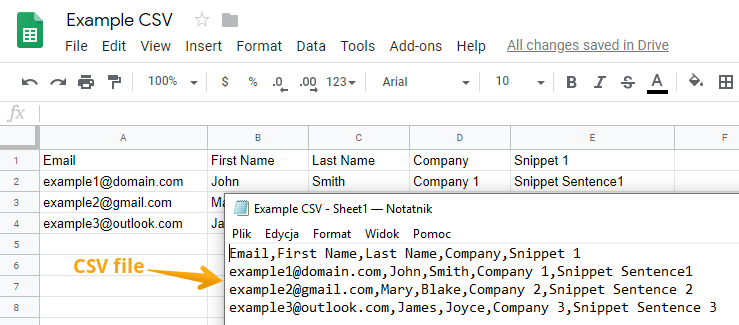
\includegraphics[width=\textwidth]{img/csv_ex.png}
\end{center}
\end{figure}

Zoals je ziet kan google sheets (of excel) de data inlezen en laten zien in rijen en kolommen, en in klablok zie je per regel de waardes gescheiden van elkaar door komma's. Dit is exact dezelfde data, alleen op verschillende manieren weergegeven. 

Als je een .csv bestand opent in bepaalde software kan het zijn dat het direct wordt herkend en de data juist wordt weergegeven, maar soms is het bestand net iets anders opgemaakt, of herkent het programma het verkeerd. Daarom is het vaak nodig om de data te importeren in plaats van te openen. Hieronder wordt uitgelegd hoe je dat in Excel moet doen. Zodra je de data hebt geimporteerd kan je het bewerken, en opslaan als fatsoenlijk .csv bestand zodat je later er mee verder kan werken.

Over het algemeen kan je in het tabblad "Data" van Excel alle opties vinden voor het importeren van gegevens. In dit tabblad vind je (afhankelijk van je versie) verschillende manieren om data te importeren. Als je data vanuit een bestand wil inlezen selecteer je de optie "Get external data -> from text"

\begin{figure}[h]
\begin{center}
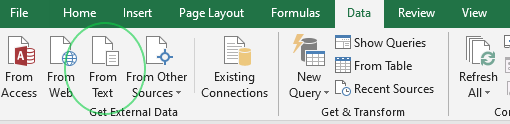
\includegraphics[width=0.5\textwidth]{img/excelimport.png}
\end{center}
\end{figure}

Selecteer nu het bestand wat je wil importeren, en daarna kom je in de \textit{Import Wizard} terecht. Hierbij helpt excel je de juiste opties te kiezen om de data te importeren. In het eerste scherm moet je kiezen of de data is gescheiden door tekens (bijvoorbeeld komma's, punten, puntkomma's, etc) of door spaties of tabs. In het scherm zie je onderin een voorbeeld van het bestand wat je wil importeren, kijk daar naar en kies de juiste optie. In het voorbeeld hieronder is de data gescheiden met puntkomma's, dus we kiezen de optie \textit{Delimited} (gescheiden door tekens, niet door spaties). Als je data ook een titel-regel heeft moet je dat ook in dit scherm aanvinken. 


\begin{figure}[h]
\begin{center}
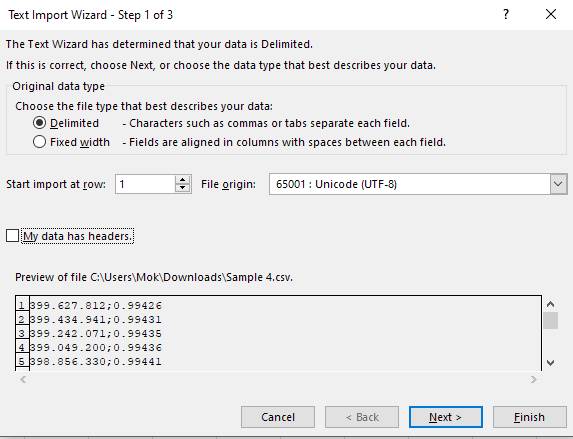
\includegraphics[width=0.5\textwidth]{img/excelimport2.png}
\end{center}
\end{figure}

Het kan ook zijn dat de data is gescheiden door komma's, maar de data ook zelf komma's bevat. Dan wordt er vaak gebruik gemaakt van aanhalingstekens om de data per cel duidelijk te krijgen, bijvoorbeeld in deze reeks waar met stapjes van een half wordt opgeteld:
\begin{verbatim}
    "0,0","0,5","1,0","1,5","2,0"
\end{verbatim}

In het volgende scherm moet je aangeven met welk teken de data is gescheiden. In dit geval zijn het puntkomma's, dus we vinken dat aan en we zien direct in het voorbeeld onderaan dat hij een streep zet tussen de twee kolommen. Als je deze streep niet ziet heeft Excel de scheiding niet goed herkend.

\begin{figure}[h]
\begin{center}
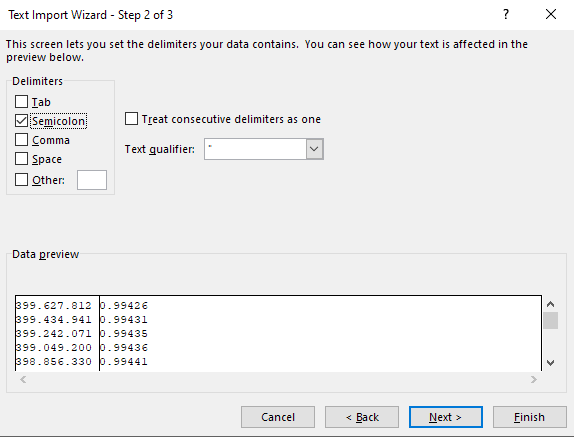
\includegraphics[width=0.5\textwidth]{img/excelimport3.png}
\end{center}
\end{figure}

In het laatste scherm kan je kiezen wat voor type data het is: een getal, tekst, datums, etcetera. Dit is vaak erg belangrijk: Excel weet niet of een punt of een komma wordt gebruikt voor getallen, dat moet je bij het knopje "advanced" aangeven. Dit is iets wat vaak wordt vergeten en veel problemen oplevert! In NL wordt er een komma gebruikt als decimaal scheidingsteken, in de VS vaak een punt. Let hier dus goed op.

\begin{figure}[h]
\begin{center}
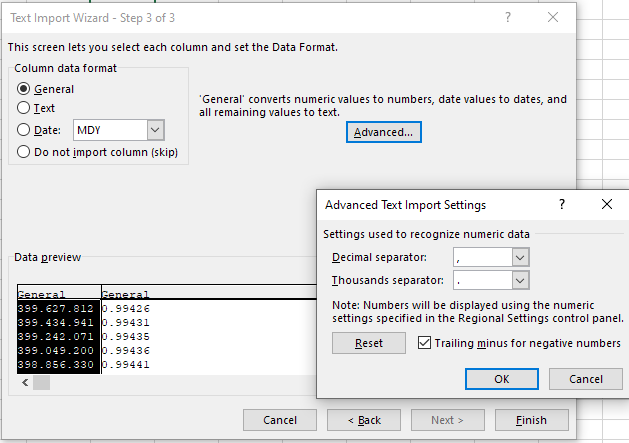
\includegraphics[width=0.5\textwidth]{img/excelimport4.png}
\end{center}
\end{figure}

Vervolgens druk je op finish, kies je waar je de data wil hebben, en klaar. Controleer dat alle data goed is overgekomen en je hebt nu alles in je excel-bestand staan!

\textbf{Opdracht (in de les):} ga naar \href{https://people.sc.fsu.edu/~jburkardt/data/csv/csv.html}{\textsf{https://people.sc.fsu.edu/$\sim$jburkardt/data/csv/csv.html}}, download minimaal 3 .csv bestanden en importeer deze in Excel. Sla op als .xlsx bestand met 3 tabbladen die de data bevatten uit de drie .csv's.

\subsection{Data bewerken en rangschikken in Excel}



TODO: Excelskills, index en match, tabellen maken, etc

\color{saxion}\textbf{Opdracht week 4: }\color{black} Gebruik de kennis die je hebt vergaard de afgelopen 2 weken om een DMP te schrijven (en uit te voeren!) voor het project Chemical Fingerprinting. De data die je verzamelt voor het project ga je volgend kwartiel gebruiken voor een automatiseringsopdracht, dus het is van belang dat je de data op een goede manier opslaat! Neem dus ook in je plan op hoe je data van de meetapparatuur gaat inlezen, omzetten en op gaat slaan. 